\chapter{Methodology}
\label{ch:solucion}
\hyphenrules{english}

OOSEM structures the development of the framework as the system of interest. Stakeholder analysis first allows an understanding of the as-is and to-be states of stakeholder capabilities. Then, this chapter presents the direct derivation of framework requirements, followed by their allocation to logical components and candidate physical architectures \citep[Chap.~17]{friedenthal2014practical}.

\section{Stakeholder Analysis}
The needs of stakeholders are analyzed by comparing the as-is state of their capabilities against a to-be (desired) state derived from a review of external references and the state-of-the-art.
This is a preliminary discussion that will be later formalized into verifiable requirements.
The analysis characterizes the needs, requirements, interfaces and technical criteria of nanosatellite EPS, both as observed within ASCEND and in the consulted references, and thus represents the deliverable of the first objective of this project.

\subsection{As-is capabilities}
For the CUBICS mission, a collaboration between ASCEND researchers and members of a student club at ÉTS is being proposed.
The present work is aimed at serving them both.

ASCEND researchers are familiar with systems engineering and even MBSE, but the nature of their position does not allow them to contribute significant time to the practical aspect of CubeSat design and development.
In contrast, ASCEND-associated students who wish to participate in CUBICS have years of experience in building systems for student engineering competitions but follow no systems engineering method.

The students have built CubeSat-format payloads for rocketry competitions, for which they verified payload power requirements only after fabrication.
This verification was observed to take the form of reusing a legacy battery pack for which the original calculations have been lost, connecting all loads, and performing mission operations repeatedly until the stored energy was depleted.
If the time until energy depletion was greater than the duration of one operations cycle as defined by the competition rules, the power requirements were taken as verified.
These experiments were reported to result in battery lifespans several times greater that one operations cycle, with the students opining that the battery pack was oversized.

In contrast, the student club members have ample experience in verifying requirements related to rocket mass, maximum height, and maximum speed before fabrication, via inspection and analysis in simulation.
These requirements are given as numerical targets by each rocketry competition, or derivated from the top-place results of previous competitions.
These competition requirements are always expressed in terms of measurable quantities, which is essential for competition grading.

ASCEND researchers report an EPS design that has been in progress for nine months.
Unclear definition of requirements has been a recurring issue, and it has forced redesigns when it is discovered that the existing requirement list is incomplete.
Requirement changes force the researchers to wait at least one week, until the next one hour-long weekly meeting, to assess their impact, because the traceability from requirements to design has to be established manually each time.

\subsection{Stakeholder concerns}
\label{sec:stakeholder-concerns}

Following OOSEM, stakeholder discussions identified concerns about the cost and effort of closing capability gaps.
These concerns inform framework requirements and measures of performance.

A project manager and systems engineer at ASCEND is concerned with maintaining verifiable requirements, redesign after fabrication, and tools suited to the team's mission scale and resources \citep[Secs.~4--5]{handpicked-0003}\citep[Sec.~1]{review-0573}\citep[Sec.~5.1]{buruso2026modelbased}.
That stakeholder is also concerned with requirement traceability, communicating verification and validation evidence, and updating EPS and other subsystem power requirements as designs change.
Maintaining consistency across requirements, models and verification evidence also demands effort \citep[Secs.~4.4 and~5.1]{buruso2026modelbased}\citep[Secs.~3--4]{review-0853}\citep[Sec.~V]{citation-0136}.

An EPS engineer is concerned with repeating verification after requirement changes, tracing design decisions, revising designs after failed verification, updating component requirements and communicating designs during technical reviews.
Further concerns include verifying safe and effective charging and power management \citep[pp.~1--3 and~6]{handpicked-0001}\citep[Sec.~3]{handpicked-0003}\citep[Secs.~5.1 and~6]{review-1251}.
Engineers responsible for other subsystems share the concern about verification cost and effort.

Taken together, the aforementioned as-is capability gaps and associated concerns can be formulated as a problem that motivates the current project:

\begin{quote}
Evidence fragmentation during the early lifecycle phases of nanosatellite electrical power systems hinders the traceability between needs and requirements, architecture decisions, and the analytical evidence that supports them. Furthermore, it hinfers the reproducibility of analyses and the capability to detect design inconsistencies before advacing to physical verification and validation phases.
\end{quote}

\subsection{Potential to-be capabilities}
After observing as-is stakeholder capabilities and recording them objectively, the OOSEM method suggests analyzing the capabilities of existing external enterprises and systems. From this, capability gaps or the lag behind the state-of-the-art can be identified and later formalized into the requirements for the systems and processes that will improve these capabilities, in this case the proposed framework.
Sources for this comparison include the academic literature, crucial for ASCEND as a research group, and normative documents.
Said sources were discussed amply in Chapter \ref{ch:marco}, to which the reader is referred in order to avoid repetition.

\section{System Requirements Analysis}
\label{section:analyze-system-requirements}
System Requirements Analysis defines how the to-be (desired) stakeholder capabilities can be obtained with support from the system of interest, the framework in this case.
The requirements define what the framework must accomplish for the stakeholders constrained by acceptable ranges of measurable system variables (Measures of Performance in OOSEM), which make them verifiable.

Table~\ref{tab:framework-requirements} gives the full list of framework requirements.
FR-01 and FR-02 establish the base unit of engineering knowledge as a requirement with forward and reverse links and quantitative values, which are used in MBSE approaches to construct a model representation of the mission.
FR-06 enables the capability to assess the impact of a change in a quantitative requirement, which is desired by the stakeholders in order to explore alternatives and keep requirements up to date in an agile manner.
FR-03 establishes that whenever an analysis is executed its inputs and outputs have to be contextualized by the mission requirements.
FR-09 establishes a controlled evolution of mission requirements and the architecture choices that depend on them, while FR-04 specifies that this evolution must be replicable without loss of information.

FR-07 and FR-08 aim to lessen the workload of inexperienced engineers, who understand EPS development from technical specifications but may struggle to follow a systems engineering line of work from high-level mission requirements, with the necessary verification measures at every step.
FR-10 and FR-11 support progress along the EPS engineering lifecycle, where early designs with ideal or assumed values must mature into evaluating the properties of real COTS.
FR-05 states that the model of what an EPS consists of, which delimits which COTS are relevant for this framework within the inmense entirety of commercial offerings, must adhere to the CSRM Profile 1.1 specification.

FR-12 to FR-20 cover fundamental analyses that are considered in the literature to be the minimum set that verifies an early EPS design and the COTS choices made for it from Phase 0 to Phase B in the NASA Reference Lifecycle. This is what the problem statement of this projects refers to as early lifecycle phases.
They cover the component types defined by CSRM and common tradeoff analyses performed at this level of design maturity.

{\small
\setlength{\tabcolsep}{4pt}
\setlength{\parskip}{0pt}
\setlength{\LTpre}{0.4\baselineskip}
\setlength{\LTpost}{0.4\baselineskip}
\renewcommand{\arraystretch}{1.06}
\begin{longtable}{@{}>{\raggedright\arraybackslash}p{0.08\linewidth}>{\raggedright\arraybackslash}p{\dimexpr0.92\linewidth-2\tabcolsep\relax}@{}}
\caption{Framework requirements.}\label{tab:framework-requirements}\\
\toprule
\textbf{ID} & \textbf{System requirement} \\
\midrule
\endfirsthead
\toprule
\textbf{ID} & \textbf{System requirement} \\
\midrule
\endhead
\bottomrule
\endfoot
FR-01 & The framework shall retain each requirement with its identifier, statement, parents and children, rationale, conditions or quantities, applicable units, verification method, and resolution status, including reasons for unresolved fields. \\
FR-02 & The framework shall retain forward and reverse links among requirements and component allocations. \\
FR-03 & The framework shall associate each analysis result with its requirement/expectation, method, scenario, parameters, raw outputs, and execution status. \\
FR-04 & The framework shall provide the inputs, dependencies and instructions to reconstruct all analyses of a mission. \\
FR-05 & The framework shall allocate EPS requirements among components covering generation, storage, conversion, regulation, protection, distribution, and control components as per the CSRM Profile 1.1 specification. \\
FR-06 & The framework shall identify impacts of a proposed mission, requirement, component, or model change on requirements and EPS design. \\
FR-07 & The framework shall recommend next engineering activities and from the current activity and inputs. identifying unmet prerequisites. \\
FR-08 & The framework shall recommend analysis, verification and validation methods or models on edits or requests using available inputs. \\
FR-09 & The framework shall retain retrievable mission states that resolve exact requirement, mission, design, and model revisions with revision history and the authorized decisions that control them. \\
FR-10 & The framework shall estimate electrical and dynamic EPS model parameters from quality-checked data. \\
FR-11 & The framework shall propose COTS EPS components from available requirements. \\
FR-12 & The framework shall calculate EPS mass and occupied volume estimates from aggregate or component data and assess margins against allocations, retaining sources, units, and unknown values. \\
FR-13 & The framework shall retain mission orbit, attitude, duration, environmental conditions, subsystem modes, and load schedules as inputs to EPS requirements and analysis. \\
FR-14 & The framework shall calculate mode-dependent power, sunlight/eclipse energy budgets, and beginning/end-of-life array and battery sizing, reporting integer cell counts, array area, and battery capacity. \\
FR-15 & The framework shall compare EPS concepts and architectures through common feasibility checks covering different choices of cell technology, reporting raw measures and unknown values. \\
FR-16 & The framework shall compare EPS concepts and architectures through common feasibility checks covering different choices of array/battery series and parallel configurations, reporting raw measures and unknown values. \\
FR-17 & The framework shall compare EPS concepts and architectures through common feasibility checks covering different choices of bus voltage and buck/boost regulation, reporting raw measures and unknown values. \\
FR-18 & The framework shall execute EPS analyses covering photovoltaic I--V/P--V characteristics against available electrical and component-rating limits. \\
FR-19 & The framework shall execute EPS analyses covering direct energy transfer vs. MPPT, against available electrical and component-rating limits. \\
FR-20 & The framework shall execute EPS analyses covering overcurrent/undervoltage/overvoltage cases. \\
\end{longtable}
}

\subsection{Measures of performance}
\label{subsection:framework-mops}

Table~\ref{tab:framework-mop-protocols} assigns Measures of Performance to the framework requirements \citep[Sec.~17.3.3]{friedenthal2014practical} to make them verifiable.
Each MOP is evaluated through one of two verification scenarios.

The first scenario reconstructs every power budget in the BIRDS-4 presentation \citep[pp.~5, 8--9, 13, 15]{shrestha2022birds4powerbudget} and the September 2019 OreSat budget \citep{oresat2019powerbudget}. The publications cited in Table~\ref{tab:framework-mop-protocols} extend these cases with mass budgets, COTS selection criteria, architecture trades, measured solar characteristics and protection tests. Each MOP in this scenario is evaluated separately for BIRDS-4 and OreSat using each mission's own published conditions. Both missions must satisfy its desired range for the MOP to pass.

For FR-12 to FR-20, expected numerical results and findings come directly from the cited publications. For each nonzero reference value $r$, the framework output $x$ must satisfy $|x-r|/|r|\leq 0.01$ after unit conversion. This 1\% tolerance applies to every numerical comparison in each mission separately. Results are not averaged across outputs or missions. Zero references require zero outputs. Component counts, series/parallel arrangements, and categorical findings require exact agreement with their references. Missing outputs fail the comparison. Source inconsistencies are reported without changing the published values.
% A missing published reference for either mission leaves that mission's comparison unverified. Evidence from the other mission does not complete the MOP.

The second scenario consists of two individual user trials, one with a PhD candidate from ASCEND and one with an undergraduate from the student club. Each participant completes the three GUI tasks in Table~\ref{tab:framework-mop-protocols} from prepared initial states. Each trial lasts 60~min, divided equally among the tasks. An evaluator prepares the task inputs and reference answers before the trials. Each GUI MOP measures elapsed time from task presentation until the saved changes and reported results match these references. Both participants must complete each task within 20~min. Incorrect or unfinished tasks are recorded as unsuccessful.

\begingroup
\small
\setlength{\tabcolsep}{4pt}
\setlength{\parskip}{0pt}
\setlength{\LTpre}{0.4\baselineskip}
\setlength{\LTpost}{0.4\baselineskip}
\renewcommand{\arraystretch}{1.0}
\setlength{\ReportTableBodyWidth}{\dimexpr\linewidth-4\tabcolsep\relax}
\begin{longtable}{@{}P{0.20\ReportTableBodyWidth}P{0.60\ReportTableBodyWidth}P{0.20\ReportTableBodyWidth}@{}}
\caption{Framework measures of performance.}\label{tab:framework-mop-protocols}\\
\hline
\textbf{MOP/FR} & \textbf{Verification protocol} & \textbf{Desired range} \\
\hline
\endfirsthead
\hline
\textbf{MOP/FR} & \textbf{Verification protocol} & \textbf{Desired range} \\
\hline
\endhead
\hline
\endfoot
\multicolumn{3}{@{}l}{\textbf{BIRDS-4 and OreSat case studies and catalogue inspection}} \\*
MOP-02/FR-02 & Retrieve forward and reverse links among the mission requirements and component allocations. Compare all linked requirement and component identifiers with the prepared mission references. & 100\% correct links \\
MOP-03/FR-03 & Inspect every budget run, including a deliberately failed run, for its linked requirement, method, scenario, parameters, available raw outputs and execution status. Compare retained records with the executed cases. & 100\% correct result records \\
MOP-04/FR-04 & Use each mission's retained inputs, dependencies and instructions to independently reconstruct and rerun all analyses in a fresh environment. Compare every output with the saved run and the applicable published reference. & $\leq 1\%$ deviation\newline All analyses reconstructed \\
MOP-05/FR-05 & Allocate each mission's EPS requirements to its catalogue components across the seven FR-05 functions. Compare component identifiers, CSRM Profile 1.1 types and allocation links with the prepared references. & 100\% correct allocations \\
MOP-06/FR-06 & Change a mission input, a requirement limit, a component and a model parameter separately. Compare affected requirement/design identifiers and updated budgets with independent dependency and calculation references. & $\leq 1\%$ deviation\newline 100\% correct impacts \\
MOP-09/FR-09 & Save both mission baselines with their revision and authorized decision records, then modify inputs and allocations. Retrieve each baseline and compare requirement, mission, design and model revisions and decision histories with the saved references. & 100\% correct baseline records \\
% FR-10: catalogue inspection verifies sourced data, not parameter estimation or dynamic model accuracy.
MOP-10/FR-10 & Present the COTS database, including components from both missions, as a table of part numbers, parameters, units, operating conditions and links to the manufacturer datasheets. Inspect each populated value against its cited page, table or curve. & 100\% correct, traceable values for both missions \\
MOP-11/FR-11 & For each mission, supply the documented selection criteria without the selected part numbers. Compare recommendations with BIRDS-4's LTC3119 choice \citep[p.~1025]{kim2021birdsbus} and OreSat's Tenergy 30005-0 and MAX17205 choices \citep{greenberg2021oresat,oresatbatteryresearch,oresat2025batterydesign}. Accept the original choice or an alternative that satisfies every documented constraint and improves the stated quantitative selection measure. & $\geq 1$ candidate per selection in each mission\newline 100\% of criteria satisfied \\
% FR-12: the OreSat budget supplies EPS subassembly masses. Its complete spacecraft mass is not an EPS mass reference.
% Published aggregate EPS mass, occupied volume and margin references remain incomplete for both missions. BIRDS-4 has no sourced aggregate EPS mass case in the selected publications.
% The 2016 OreSat mass budget also contains inconsistent line sums and an approximate spacecraft margin. Preserve these source discrepancies.
MOP-12/FR-12 & For both missions, calculate EPS mass, occupied volume and margins against allocations. Compare each result with a published reference at the same component boundary, including OreSat's 252~g solar module and 416~g battery module entries \citep[Sec.~D.2]{oresat2016csli}. Check retained sources, units, unknown values and margin findings for each mission. & $\leq 1\%$ per mission\newline Exact records and findings \\
MOP-13/FR-13 & For BIRDS-4 and OreSat, enter and save orbit, attitude, duration, environment, modes and load schedules from their published mission records \citep{jara2022birdsepsdataset,oresat2019powerbudget}. Reopen each mission and compare retained fields and analysis inputs with its own source values. & $\leq 1\%$ per mission\newline Exact categorical inputs \\
% FR-14: the budgets verify reported energy and storage calculations. Full mission BOL/EOL array and battery sizing and installed array area lack published output references for both missions.
MOP-14a/FR-14 & Recalculate all published load and generation rows, mode totals, storage capacities, battery configurations, recharge times and payload pass counts for both missions using their original quantities, duty cycles and margins. Compare every output separately with its mission's published value. & $\leq 1\%$ per mission\newline Exact counts and arrangements \\
MOP-14b/FR-14 & Reproduce the BIRDS-4 worst-case budgets with 1604, 1202 and 801~mWh available at the load and the deficit against 1438~mWh nominal consumption \citep[Tables~2--4]{shrestha2022birds4powerperformance}. Reproduce OreSat's 1011~mWh standby energy surplus \citep{oresat2019powerbudget}. Compare energy quantities and balance findings separately for both missions. & $\leq 1\%$ per mission\newline Exact published findings \\
% FR-15: the 2026 BIRDS-4 hybrid result is a proposed configuration simulated with sun tracking, not a flown BIRDS-4 configuration or its original free-rotation budget.
% The article also mentions free rotation and gives a generic physical-parameter table from a 6U study. Resolve the applicable published inputs before claiming 1% reproduction of its BIRDS-4 result.
MOP-15/FR-15 & Compare published cell technology alternatives for both missions. Reproduce the BIRDS-4 hybrid solar case with ten triple-junction and six monocrystalline cells and 3.023~Wh per orbit \citep[Sec.~III]{shrestha2026solarreliability}. Repeat OreSat's lithium-ion, lithium iron phosphate and lithium titanate trade \citep{oresatbatteryresearch}. Compare each mission's energies, capacities and selection findings under its published conditions, retaining unknown properties. & $\leq 1\%$ per mission\newline Exact published findings \\
% FR-16: BIRDS-4 baseline arrangements are sourced. Published alternative arrangement cases and their feasibility findings remain needed for complete BIRDS-4 comparison coverage.
MOP-16/FR-16 & For each mission, compare array and battery series/parallel choices with published counts, capacities and selection findings. Include BIRDS-4's two-cell solar strings and 3S2P, 3800~mAh battery \citep[Sec.~2.2, Table~5]{shrestha2021birdssafety}, OreSat's two independent 2S packs and 37.4~Wh per card \citep[p.~6]{greenberg2021oresat}, and its 74.88, 86.4 and 64.8~Wh alternatives against 80~Wh \citep{oresatbatteryresearch}. & $\leq 1\%$ per mission\newline Exact counts, arrangements and findings \\
MOP-17/FR-17 & For each mission, compare bus voltage intervals, buck/boost functions and feasibility findings with published cases. Check BIRDS-4's 3.3 and 5~V regulated lines \citep[Sec.~2.2.3]{shrestha2021birdssafety} and OreSat's 1S, 2S and 4S bus choices and SPV1040 rejection after the change from 1S to 2S \citep{oresatbatteryresearch,oresatsolarhistory}. & $\leq 1\%$ per mission\newline Exact published findings \\
% FR-18 compares labelled graph values and published spreadsheet outputs. Unlabelled coordinates do not receive an assumed 1% reading accuracy.
% Empirical I--V samples support numerical reconstruction. Reusing those samples as both model inputs and prediction references does not validate a physical cell model.
MOP-18/FR-18 & Reconstruct the BIRDS-4 Maya-2 +Z panel I--V/P--V characteristics and compare labelled voltages, powers and the 1.575~W peak with the published curves \citep[Figs.~13--14]{shrestha2021birdssafety}. Reconstruct OreSat's measured solar sweep and compare calculated power with its published spreadsheet values \citep{oresatsolarsweep}. Check each mission's labelled or tabulated values separately. & $\leq 1\%$ per mission \\
% FR-19: no published paired DET/MPPT case was found for either mission. Both missions still need sourced numerical cases for this MOP.
% BIRDS fixed input-voltage control and OreSat's regulated constant-voltage fallback are not DET references.
MOP-19/FR-19 & For BIRDS-4 and OreSat separately, compare DET and MPPT using published paired cases with identical array, battery, illumination and load conditions. Compare delivered energy, operating points, conversion losses and electrical-limit findings with that mission's published results. & $\leq 1\%$ per mission\newline Exact published findings \\
% FR-20 checks steady-state overvoltage protection, static currents, protection settings and state logic. A published BIRDS-4 undervoltage protection case is still missing, and these sources do not establish transient fault response accuracy for either mission.
MOP-20/FR-20 & For both missions, check overcurrent, undervoltage and overvoltage cases against published outputs and protection findings. Include BIRDS-4's BCR test with input at or above 4.8~V and output near 4.2~V \citep[Sec.~3.6]{shrestha2021birdssafety} and its 2, 3 and 4~A line thresholds \citep[Sec.~6.3]{kyutech2021birdsicd}. Check OreSat's 30~W load currents and charge/discharge disable and recovery criteria \citep{oresat2025batterydesign}. & $\leq 1\%$ per mission\newline Exact published protection findings \\
\multicolumn{3}{@{}l}{\textbf{User trials}} \\*
MOP-01/FR-01 & Given a fully defined mission requirement, create another requirement with the FR-01 fields filled in and a simple verification condition, reopen it, and report its retained fields and condition result. & $\leq 20$~min \\
MOP-07/FR-07 & Given complete mode allocations and load powers with eclipse duration omitted, request the next activity and identify the unmet prerequisite. Supply that duration and report the updated recommendation. & $\leq 20$~min \\
MOP-08/FR-08 & Given an EPS requirement and its supporting inputs, request analysis, verification and validation recommendations and report the suggested methods or models. & $\leq 20$~min \\
\end{longtable}
\endgroup

\section{Define Logical Architecture}
\label{section:define-logical-architecture}

Nine logical components realize F01--F08 without specifying implementation technologies \citep[Sec.~17.3.4]{friedenthal2014practical}. Learning, finances, RAM, credibility, software and technician concerns extend the response beyond evidence custody. El Hachimi et al. inform mission-driven sizing, component and thermal/EMC decisions, protection and telemetry checks \citep[Secs.~2--5 and~8.1.6--8.1.7]{handpicked-0003}. The Handbook informs coordinated requirements, budgets, interfaces and verification planning \citep[Secs.~I.3--I.4]{aguado2021cubesatse}. Their EPS results remain case-specific.

\subsection{Responsibilities and allocations}

Figure~\ref{fig:framework-logical} presents three views of the same nine logical components, with their important records, required information and provided services. Each dashed reference refers to an existing component, not an additional component or deployment. FR numbers identify the 40 primary responsibility allocations. Supporting responsibilities and exchanges remain formalized in the SysML v2 model. This decomposition imposes no executable or node count. Intended allocation is not demonstrated requirements satisfaction \citep[Sec.~17.3.7]{friedenthal2014practical}.

% One figure, continued across three pages to keep the native summaries readable.
\begin{figure}[p]
\centering
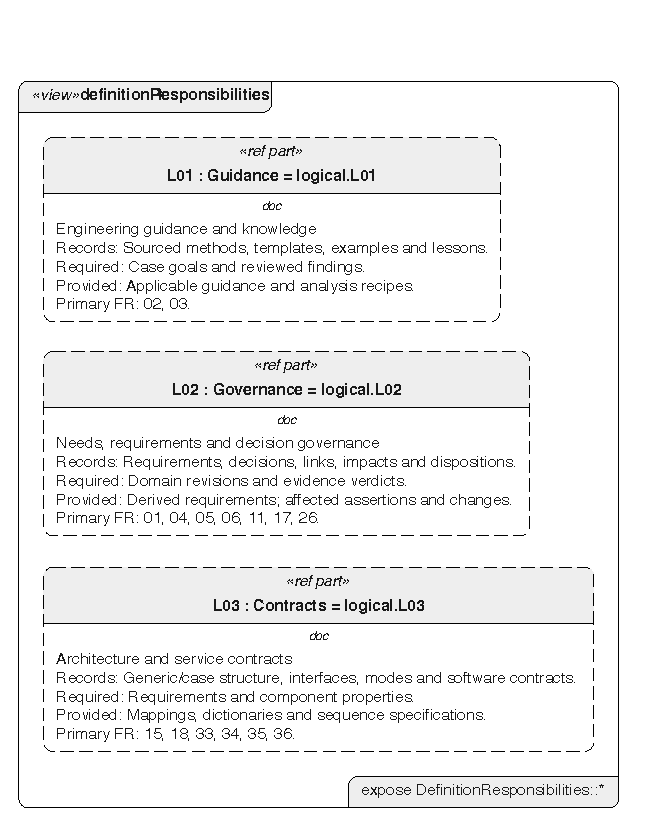
\includegraphics[width=\linewidth,height=0.84\textheight,keepaspectratio]{fig/sysml/logical/sysml-defined-view-logicalresponsibilityviews-definitionresponsibilities.pdf}
\caption{Logical component responsibilities, records and required/provided services. Primary FR numbers state intended allocation, not demonstrated satisfaction. (a) L01--L03: guidance, governance and architecture.}
\label{fig:framework-logical}
\end{figure}
\begin{figure}[p]
\ContinuedFloat
\centering
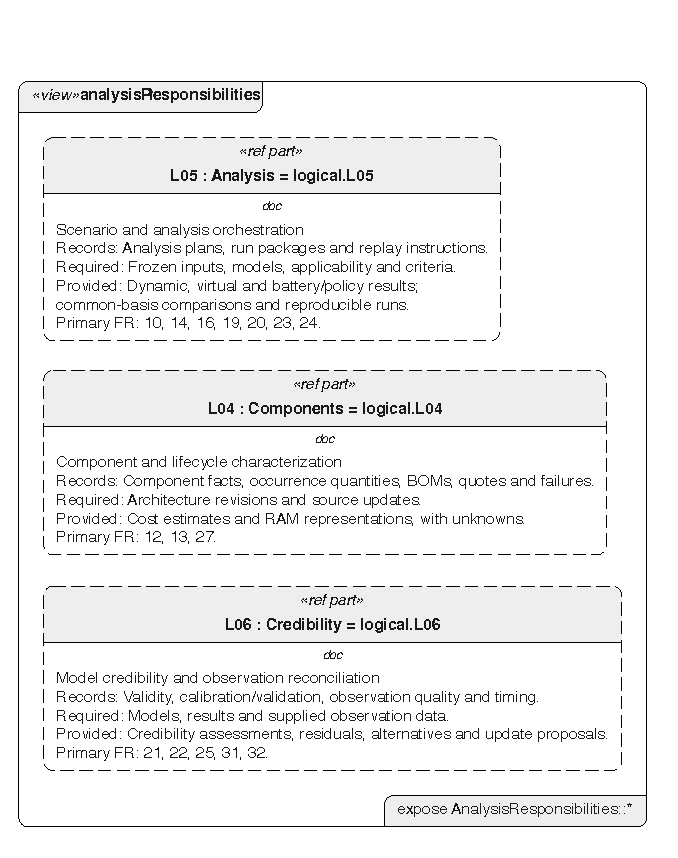
\includegraphics[width=\linewidth,height=0.84\textheight,keepaspectratio]{fig/sysml/logical/sysml-defined-view-logicalresponsibilityviews-analysisresponsibilities.pdf}
\caption[]{Logical component responsibilities (continued). (b) L04--L06: characterization, analysis and credibility.}
\end{figure}
\begin{figure}[p]
\ContinuedFloat
\centering
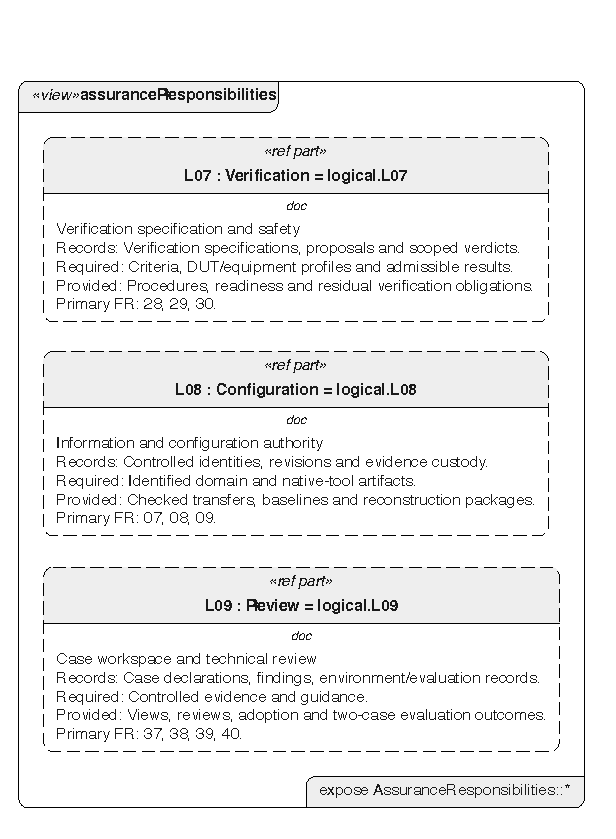
\includegraphics[width=\linewidth,height=0.84\textheight,keepaspectratio]{fig/sysml/logical/sysml-defined-view-logicalresponsibilityviews-assuranceresponsibilities.pdf}
\caption[]{Logical component responsibilities (continued). (c) L07--L09: verification, configuration and review.}
\end{figure}
\clearpage

\subsection{Typed exchanges, authority and feedback}
{\small
\setlength{\tabcolsep}{4pt}
\setlength{\parskip}{0pt}
\setlength{\LTpre}{0.4\baselineskip}
\setlength{\LTpost}{0.4\baselineskip}
\renewcommand{\arraystretch}{1.06}
\begin{longtable}{@{}>{\raggedright\arraybackslash}p{\dimexpr0.32\linewidth-0.64\tabcolsep\relax}>{\raggedright\arraybackslash}p{\dimexpr0.68\linewidth-1.36\tabcolsep\relax}@{}}
\caption{Information exchanges between logical components.}\label{tab:framework-logical-exchanges}\\
\toprule
\textbf{Participants} & \textbf{Exchanged information and required handling} \\
\midrule
\endfirsthead
\caption[]{Information exchanges between logical components. (continued).}\\
\toprule
\textbf{Participants} & \textbf{Exchanged information and required handling} \\
\midrule
\endhead
\bottomrule
\endfoot
All $\leftrightarrow$ L08 & Registration, transfer verdict, exact manifest and reconstruction. Check envelope/semantics/provenance and preserve rejected/prior revisions. \\
L02 $\leftrightarrow$ L03/L04/L06/L07 & Requirements, criteria, impact and domain revision proposals. Resolve dependencies and retain stale/unresolved evidence. \\
L03/L04/L06/L07 $\rightarrow$ L05 & Occurrences, characterization, failure dependencies, applicable models and verification criteria freeze the run. Software mappings also drive sequence/resource checks. \\
L05 $\rightarrow$ L06 $\rightarrow$ L07 $\rightarrow$ L02 & Raw analysis results, model credibility assessment, verification verdict based on admissible evidence and status of affected technical assertions. Supplied observations return through proposed parameter/design updates. \\
L01/L09 $\leftrightarrow$ domain owners & Guidance, baseline-linked reviews, findings and lessons. Apply tailoring, return findings to owners and separate local learning from general source claims. \\
\end{longtable}
}

L08 controls accepted baselines and consistent identification. Each domain component remains responsible for the meaning of its information: requirements (L02), architecture and interfaces (L03), component characteristics (L04), models and observations (L06), verification (L07), knowledge (L01) and case reviews (L09). Generated analysis inputs, software definitions and views refer to these controlled sources rather than creating competing definitions. Mission software behavior and deployment still require separate implementation and verification \citep[Secs.~3--5]{review-0853}.

Interface specifications for quantities, signs, reference frames, clocks and validity address model, degradation, sensor and timing effects \citep[Secs.~4.1--4.2 and~6]{review-1251}. Numerical step size proves no real-time suitability \citep[Sec.~3]{review-0573}. SC01 follows guidance and definition, analysis, credibility assessment, verification and review. SC02 evaluates change impacts through domain revisions and reanalysis. SC03 uses failed checks or supplied observations to propose updates and safe verification activities. Design change, observation reconciliation and reviewed learning share L08 revision control. They never silently overwrite earlier evidence or actuate hardware.

\section{Synthesize Candidate Physical Architectures}
\label{section:synthesize-physical-architectures}

The physical architecture identifies the software, persistent data, operating procedures and computing resources that realize the eight logical responsibilities. OOSEM first partitions responsibility, information and control across logical nodes. It then allocates them to physical components and hosts, with explicit interfaces and component specifications \citep[Sec.~17.3.5]{friedenthal2014practical}. This is the framework architecture. EPS arrays, batteries, converters and controllers remain engineered model/software products.

\subsection{Partitioning and common scope}

Three logical nodes group the current responsibilities. The \emph{engineering node} contains exchange, requirements, design, analysis, credibility and review (L01, L03--07). The \emph{assistance node} contains L02. The \emph{evidence node} contains configuration and currency (L08). These groups separate interactive drafting from long numerical work and separate editable working records from preserved releases. They describe responsibilities rather than a fixed number of computers.

{\small
\setlength{\tabcolsep}{4pt}
\renewcommand{\arraystretch}{1.06}
\begin{longtable}{@{}>{\raggedright\arraybackslash}p{0.30\linewidth}>{\raggedright\arraybackslash}p{\dimexpr0.70\linewidth-2\tabcolsep\relax}@{}}
\caption{Physical partition decisions and their measures.}\label{tab:framework-partitioning}\\
\toprule
\textbf{Criterion} & \textbf{Consequence and current basis} \\
\midrule
\endfirsthead
\toprule \textbf{Criterion} & \textbf{Consequence and current basis} \\
\midrule
\endhead
\bottomrule
\endfoot
Meaning and authority & Keep requirement, design and evidence meanings with L03, L04 and L06--07. L08 preserves their exact revisions. Assign one owner per field. MR-02--05, MOE-02--03, MOP-03--05. \\
Interactive response & Run assistance independently of numerical execution. Invalidate guidance immediately on edits. Record pending/unavailable work. MR-02 and 05, MOE-01 and 04, MOP-01--02 and 04. \\
Replaceable analysis & Declare discipline, model, solver and host profiles at the analysis boundary. Verify every mandatory profile. Separate execution from credibility and EPS assessment. MR-03--04, MOE-02--03, MOP-03 and 05. \\
Access and preservation & Keep private engineering inputs local by default. Preserve sources, raw results and released dependencies with backup/restore. Verify external access, exports and recovery. MR-05, MOE-03--04, MOP-04--06. \\
Adoption and variation & Separate reusable rules, libraries and methods from mission inputs and model/software products. Compare correct-task effort and dated framework cost. MR-01--05, MOE-01 and 04, MOP-06. \\
\end{longtable}
}

Every complete candidate specifies the same 41 FRs, eight logical responsibilities and Pre-Phase A through adapted C tasks. Each includes active drafting assistance, explained contextual recommendations, EPS modeling, applicable discipline/RAM analysis, credibility, controlled changes and reviews. An external declared host toolchain codes, builds and executes SIL only after the exact current engineer-authorized detailed design/interface release. Generic computing hosts are framework infrastructure. Physical EPS realization, procurement, testing, PIL/HIL and flight readiness remain excluded.

\subsection{Five coherent configurations}

Five configurations provide distinct authoring and collaboration arrangements. These are COMET and Excel (PA-COM), SysML and Python (PA-CDT), YAML and Git (PA-GY), Nanospace (PA-NS), and Capella and Valispace (PA-VS). Shared proposed assistance and analysis components make their scope comparable. Source-supported workflows establish reusable mechanisms. They establish neither complete EPS readiness nor implemented framework compliance.

{\small
\setlength{\tabcolsep}{4pt}
\renewcommand{\arraystretch}{1.07}
\begin{longtable}{@{}>{\raggedright\arraybackslash}p{0.14\linewidth}>{\raggedright\arraybackslash}p{\dimexpr0.43\linewidth-2\tabcolsep\relax}>{\raggedright\arraybackslash}p{\dimexpr0.43\linewidth-2\tabcolsep\relax}@{}}
\caption{Five complete candidate configurations. All additions require development and verification.}\label{tab:framework-candidate-inventories}\\
\toprule
\textbf{Candidate} & \textbf{Configuration and reason to retain} & \textbf{Proposed additions and important limits} \\
\midrule
\endfirsthead
\toprule \textbf{Candidate} & \textbf{Configuration and reason to retain} & \textbf{Proposed additions and important limits} \\
\midrule
\endhead
\bottomrule
\endfoot
PA-COM & COMET server, desktop client and Excel add-in provide parameter ownership, catalogues and budget calculations. Retain this concurrent engineering arrangement \citep[Secs.~3--4]{deutsch2022comet}. & Python companion requirement/trace records, edit-linked assistance, analysis, credibility, reviews and Git/archive releases. COMET parameters are linked to requirement meaning. Current API/add-in compatibility, Excel rights and workbook reconstruction are unresolved. \\
PA-CDT & Native SysML v2 authoring and views through Syside, Python engineering calculations, Git and a managed archive. Retain explicit local model authority and replaceable tools. CSRM supplies structural patterns \citep{kaslow2019csrm}. & A native EPS library, authoring assistance panel, analysis/profile mappings, impact checks and assessment services are proposed. CSRM is not a completed SysML v2 migration. Deployment licence, authoring API, quantities, capacity and clean reconstruction need proof. \\
PA-GY & Typed YAML engineering definitions, Git review, an editor/Python assistance panel and generated views. Retain portable reviewable text \citep{kanavouras2024lightweight,chiu2023sealion}. & Develop engineering units/relationships, requirement allocation, assistance, analyses, credibility and authority controls. The lightweight source excludes requirement/test management. Git history supplies no technical approval. Contributor usability is unresolved. \\
PA-NS & Nanospace browser/API parameter collaboration, declared native model authority, Python services and Git/archive releases. Retain concurrent sharing and dependency analysis \citep[Secs.~3--6]{review-0340}. & Add active browser assistance, requirement semantics, controlled exports and full analysis/assessment services. HyperTension/HDDL planning is an optional proposed adapter. Integrated planning is future work. Gaphor extraction is a separate tool-specific option \citep{luccisano2024formalization}. \\
PA-VS & Capella/ARCADIA owns structure, allocations, modes and interface meanings. Valispace owns requirements, properties and budgets. Python for Capella and REST transfers connect them \citep[Secs.~3--4]{campioli2025integration}. & Add edit-linked assistance, stable-ID reviewed transfers, dynamic analysis, credibility and Git/archive releases. Demonstrated preliminary tree/mode/budget transfers support retention. Current service access, deletion/conflict handling, exports and reconstruction remain unresolved. \\
\end{longtable}
}

Each candidate deploys its engineering services on a generic workstation and any declared authoring server, local assistance on an independently scheduled process, and identified releases/raw outputs on a managed archive. These roles can share hardware if access, response, numerical workload and recovery limits are met. Versions, CPU, memory, storage, network, operating system, licences and backup arrangements must be declared before deployment. No capacity or licence price is assumed.

\subsection{Active assistance realization}
\label{subsection:physical-assistance}

The service retrieves relevant engineering sources, ranks candidate findings or methods, and prepares cited explanations for engineer assessment.

Every candidate includes the following proposed Python service. Its attachment point is the COMET/Excel editor, native model workbench, YAML editor, Nanospace browser or Valispace/Capella workspace. An edit is acknowledged and invalidates affected current and pending guidance before delayed work starts. The service captures the exact requirement, mission, design, source, criterion and scope revisions.

\paragraph{Rules, selection and ranking.}
Versioned structural, quantity and wording rules check required fields, identifiers, parents, responsible product, modal wording, single obligations, units, inequalities and declared numerical limits. NASA Appendix C and an expert-approved project reference supply the default criteria \citep[Sec.~4.2 and Appendix~C]{nasa2016systems}. Broad semantic findings remain probable. For example, ``battery capacity: 200 W'' triggers a dimensional finding and a question about the intended quantity. It cannot justify inventing ``200 Wh''.

Source selection preserves authority and citation metadata while selecting substantive passages, tables, equations and necessary context. BM25 retrieves candidate passages through lexical ranking against the query terms. Local \texttt{Qwen3-Embedding-0.6B} retrieves semantic candidates, and \texttt{Qwen3-Reranker-0.6B} scores query/passage pairs \citep{qwen3embedding,qwen3reranker}. Their proposed initial revisions are respectively \texttt{97b0c614be4d} and \texttt{e61197ed4502}. The native specification retains the full revisions. Tokenizer, prompts, library versions and input limits also require control. Separate content and contextual relevance rubrics require qualification. Necessary standards passages cannot disappear silently through a content filter.

Pinned \texttt{jev-1.13.0} through TypeSafe SDK 0.6.0 is an alternative for substantive-content and current-question relevance scoring \citep{typesafe060}. Structured requirement-pair similarity/conflict questions are a proposed additional use. Existing passage reranking is pointwise. Noul scores return neither explanations nor corrections. Requested and returned model identities must agree with the qualified profile. A changing ``latest'' alias is excluded. Local Qwen/BM25 offers data locality and offline operation, with resource and domain-qualification costs. Jev offers an external scoring service, with unresolved access, privacy, cost, outage and qualification dependencies. Neither option demonstrates technical correctness.

Method/model options first pass mandatory scope, purpose, input, fidelity, validity, resource and access checks. Unknown prerequisites remain unresolved. Only eligible options enter shortlist ranking. Duplicate candidates compare level, subject, mode, conditions, quantity and parent allocation. Similar statements can be valid separate requirements. Coverage uses a declared ConOps/function/interface/risk set. Corpus retrieval cutoffs and score-fusion weights supply no engineering acceptance limit. Project limits, ranking criteria and abstention rules require independent expert qualification against the current MOPs.

\paragraph{Separate explanations and controlled use.}
The explanation component combines identified rule templates, cited source excerpts and explicit comparisons of engineering context. It shows affected text, observed quantities, applicable conditions, legitimate differences, alternatives and rejection reasons. It proposes corrections or clarification questions. Conflicting source limits remain separate until an engineer resolves authority and applicability. This mechanism needs no text generator. Any later generator needs a pinned identity and separate source fidelity qualification.

Insufficient context, decisive truncation, unsupported language, uncertain applicability, invalid scores or unavailable services produce flags or abstention. No eligible recommendation remains an explicit result. Unassessed scope differs from a completed check with no finding. Source text is evidence and cannot issue instructions to the framework. Engineers retain accepted, modified, rejected and deferred dispositions. Currency is checked against the latest revisions before display and again before authorized application.

Remote processing requires approved data rights, minimized payloads and declared retention. Private inputs remain local by default. Request count, concurrency, spend, retries and total response time are bounded by the approved workload/profile. Outage leaves deterministic checks available. A separately qualified local profile may supply semantic results. Otherwise that assessment is unavailable. Caches retain question, source/context, rule/rubric, requested/returned model and qualification revisions. Superseded entries remain historical and cannot become current advice. No current API price or availability is asserted.

\subsection{EPS analysis tools and model fidelity}

Engineers need progressively refined sizing, time-dependent energy analysis and battery assessment. The tools below support those decisions through a common mission and design basis.

The configurations share a controlled analysis boundary. A proposed CPU starting profile combines transparent Python sizing/budget equations, time-dependent EPS/control models informed by Casado, and PyBaMM when battery electrochemical, thermal or aging detail is justified. Orbit, attitude, illumination, load and mode histories use the same controlled mission/design basis. Casado's published model structures are transferred as design information. A host numerical implementation is proposed, with no reuse of its executing HIL equipment \citep[Secs.~2--4]{review-0573}.

Boan's tool chain is an alternative complete preliminary analysis profile: IDM-CIC defines the system/geometry and budgets, Simu-CIC generates scenario ephemerides, IDM-Power forms temporal demand, Flows Manager converts ephemerides into incident fluxes, and Opalis models generation/storage/distribution and energy balance. Their linked inputs and outputs explain how the profile integrates, rather than forming a list of disconnected tools. The paper calls the tools non-compulsory and Opalis proprietary but open. Current access and transfer compatibility remain unknown \citep[Secs.~2--4]{review-0289}.

GREATCUBE+ is an optional concept-seeding profile. Its empirical, analytical/COTS and numerical placement levels supply progressively refined starting designs. Those outputs require source checks and mission adaptation before entering L04. It excludes price/availability from component trade-offs, uses limited heritage correlations and treats downstream electrical simulation as future work. It supplies no EPS acquisition or framework cost result \citep[Secs.~2--4]{review-0711}.

Gateau's dependency graph/DSM and curated HDDL/HyperTension methods can refine activity recommendations from prerequisites and impacts. Its planning demonstration is separate from Nanospace integration and returns a valid plan rather than an optimum. Campioli's tree/mode/budget transfers support PA-VS interfaces. Its broader AIV/T extension remains prospective \citep[Secs.~3--6]{review-0340} \citep[Sec.~6]{campioli2025integration}.

Zhu supports a conditional PyBaMM SPM/DFN and thermal/calibration profile using supplied data. PhysicsNeMo surrogates require suitable training data, independent assessment, uncertainty and intended-use justification. Omniverse/OpenUSD is an optional geometry view only when illumination, accommodation or thermal decisions need it. No mandatory 3D, Isaac, autonomous control or live feedback is inherited. Geometry supplies no electrical fidelity \citep[pp.~7--9]{handpicked-0001}.

Electrical, thermal and every applicable EMC/geometry profile require verified mappings, units, time bases, numerical checks, supported effects and independent reference evidence. A declared specialist tool or transparent analysis is selected for each required question. No source establishes a complete EMC implementation here. Averaged or lossless converters cannot support switching-spectrum/loss claims. Casado omits PV degradation, fixes battery temperature/SOH and simplifies loads. These limits require explicit restrictions or verified extensions. Missing mandatory discipline capability blocks the affected complete-use claim.

RAM transformations retain identified functions/components, dependencies, assumptions, missing failure/repair data and uncertainty. Calibration retains prior/revised parameters, supplied-data identity and residual units. Independent assessment stays separate. All profiles preserve raw histories, invalid/missing samples, masks, sample/receipt times, solver settings, resources, failures and partial results. cFS and F-Prime are optional engineer-selected host integration mappings, each requiring verification. Corresponding MIL/SIL runs use matched stimuli and fixed comparison rules. Successful execution or replay establishes no framework V\&V, predictive validity or EPS readiness.

